\chapter{المشاريع والتخطيط}
\label{ch:projects}

\section{ماذا ستنجز؟}

ينظم تطبيق المشاريع العمل الذي يحتاج إلى خطة وموارد ونتائج يمكن مراجعتها. يحدد المسؤول الإعدادات والصلاحيات، ويضع مدير العمل الخطة ويتابع التنفيذ، ويحدّث الموظف السجلات المسندة إليه. ابدأ بالخطة عندما تحتاج إلى تحديد توجه أو نتيجة، وبالمشروع عندما يكون لديك عمل محدد النطاق تريد تسليمه.

\begin{rcnote}[مثال: شركة الأفق]
تستخدم سارة الخطيب خطة لتحسين جاهزية زيارات شركة الأفق، وتتابع مشروع تجهيز زيارة فرع حلب. يعدّ عمر حداد ملف الزيارة، ثم تراجع سارة المخرجات قبل اعتبار التحضير مكتملاً.
\end{rcnote}
\begin{figure}[H]
\centering
\begin{tikzpicture}[node distance=0.5cm]
\node[stepBox] (n0) {\RL{تحديد النتيجة والمسؤولية}};
\node[stepBox,below=of n0] (n1) {\RL{تهيئة العمل واعتماده}};
\node[stepBox,below=of n1] (n2) {\RL{التنفيذ والمراجعة}};
\draw[flowsTo] (n0) -- (n1);
\draw[flowsTo] (n1) -- (n2);
\end{tikzpicture}
\rclegend
\caption{من النتيجة المطلوبة إلى مراجعة التنفيذ}
\label{fig:projects-overview}
\shotnote{يضع المخطط تحديد النتيجة والمسؤولية قبل التنفيذ، ثم يربط المتابعة بما تحقق فعلياً. لا يعني هذا التسلسل أن إنشاء خطة ينشئ مشروعاً أو يوافق عليه تلقائياً؛ لكل سجل إجراءاته ومسؤوليته.}
\end{figure}

المحفظة تجمع برامج ومشاريع لخدمة أولويات مشتركة، والبرنامج ينسّق مشاريع مترابطة. هذه الروابط اختيارية في تعريف المشروع؛ لا تنشئ محفظة أو برنامجاً لمجرد الوصول إلى صفحة المشاريع. وتختلف الخطط والمشاريع هنا عن تبويب المهام الكبرى داخل تطبيق المهام.

\section{دليل صفحات المشاريع والتخطيط}
\label{sec:projects-pages}
\begin{figure}[H]
\centering
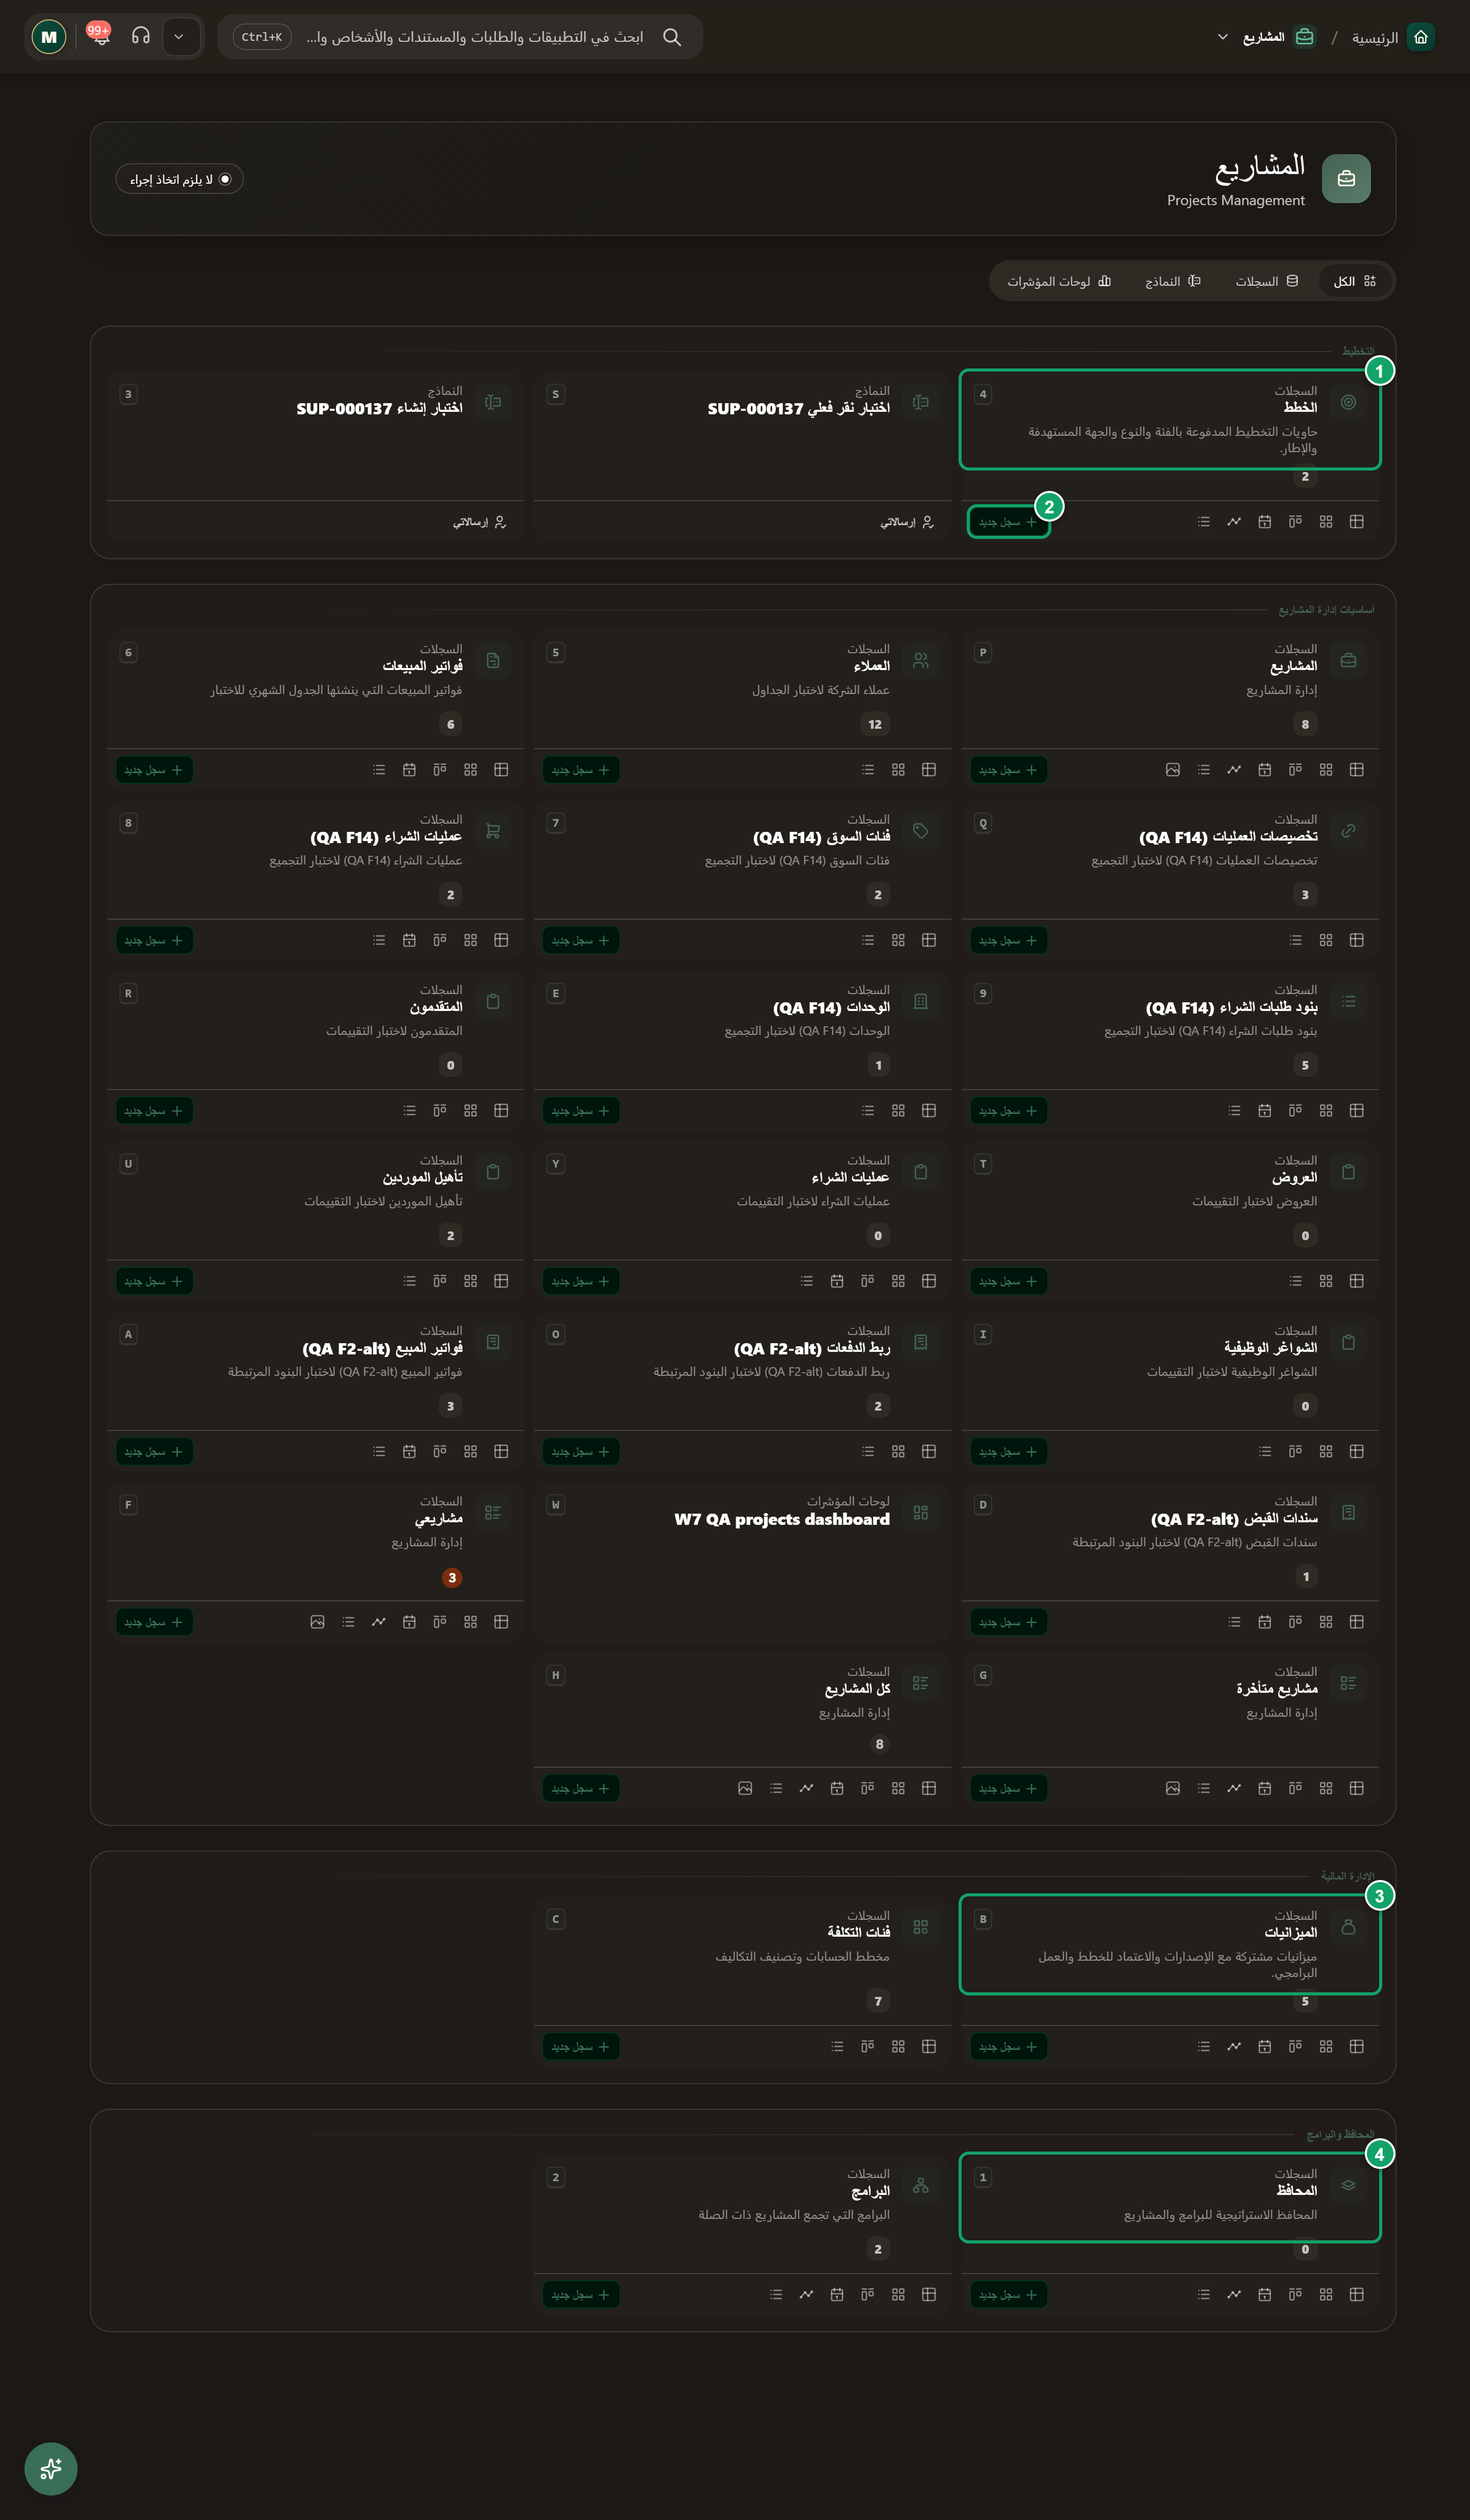
\includegraphics[width=0.95\linewidth,height=0.72\textheight,keepaspectratio]{figures/screens/ch05-directory-ar.png}
\caption{مدخل تطبيق المشاريع في بيئة الاختبار}
\label{fig:projects-screen-directory}
\shotnote{تعرض بطاقات التطبيق الصفحات الست الأساسية والعروض المخصصة المتاحة للحساب. العروض مثل المشاريع المسندة إليّ تعرض سجلات المشاريع نفسها، وليست نوعاً جديداً من السجلات؛ وقد تختلف البطاقات والأعداد باختلاف الصلاحيات والنطاق المختار. ① بطاقة «الخطط» تفتح قائمة الخطط. ② «سجل جديد»: ينشئ سجلاً مباشرة من البطاقة دون فتح القائمة. ③ بطاقة «الميزانيات» في قسم الإدارة المالية. ④ بطاقة «المحافظ» في قسم المحافظ والبرامج.}
\end{figure}

ابدأ بالصفحات الرئيسية، ثم افتح شرح السجل الذي تحتاج إليه من المجموعات التالية. بقية الصفحات تشرح سجلات أو أدوات داخل تبويبات، وليست كلها مداخل مستقلة في قائمة التطبيق. استخدم البحث والفلاتر والعروض المتاحة في القوائم للوصول إلى السجل؛ ولا تغيّر الفلاتر السجل نفسه.
\begin{table}[H]
\centering
\caption{الصفحات الرئيسية}
\label{tab:projects-pages-foundations}
\begin{tabularx}{\linewidth}{R{4.2cm} Y}
\rcHeaderRow
\thh{الصفحة} & \thh{ماذا تقدم هذه الصفحة؟}\\
الخطط & تجمع الخطة النتيجة المطلوبة والجهة المسؤولة والفترة التي ستعمل خلالها.\\
المشاريع & يجمع المشروع عملاً محدد النطاق له مدير ونتيجة مطلوبة.\\
المحافظ & تجمع المحفظة برامج ومشاريع تخدم توجهاً مشتركاً، وتساعد الإدارة على مراجعة الأولويات والتمويل.\\
البرامج & ينسّق البرنامج مشاريع مترابطة لتحقيق فائدة مشتركة.\\
الميزانيات & تجمع الميزانية بنود التكلفة ومصادر التمويل والمصروفات في سجل واحد.\\
فئات التكلفة & توحّد فئات التكلفة طريقة تصنيف بنود الميزانية، مثل السفر والتجهيزات.\\
\end{tabularx}
\end{table}
\begin{table}[H]
\centering
\caption{الأهداف والنتائج}
\label{tab:projects-pages-direction}
\begin{tabularx}{\linewidth}{R{4.2cm} Y}
\rcHeaderRow
\thh{الصفحة} & \thh{ماذا تقدم هذه الصفحة؟}\\
المحاور التخطيطية & يجمع المحور الاستراتيجي مجموعة من الأولويات تحت توجه واضح.\\
أهداف التخطيط & يصف الهدف التغيير الذي تريد الخطة تحقيقه.\\
المبادرات التخطيطية & تسجّل المبادرة عملاً مقترحاً يدعم التوجه الاستراتيجي.\\
دورات OKR & تجمع دورة الأهداف والنتائج الرئيسية أهداف فترة محددة والنتائج التي تقيس تحققها.\\
النتائج الرئيسية & تحوّل النتيجة الرئيسية الهدف إلى نتيجة قابلة للمتابعة.\\
متابعات النتائج الرئيسية & يسجّل تحديث النتيجة الرئيسية وضعها في تاريخ محدد.\\
عناصر هوشين & يربط أسلوب هوشين التوجهات طويلة المدى بالأهداف السنوية والعمل المطلوب.\\
روابط مصفوفة X لهوشين & توضح روابط مصفوفة هوشين كيف يدعم عنصرٌ عنصراً آخر.\\
تبادلات كاتشبّول لهوشين & تسجّل جولات التشاور المقترحات والردود حول عنصر من عناصر هوشين.\\
الإجراءات المضادة لهوشين & يسجّل الإجراء التصحيحي استجابةً لتعثر عنصر من عناصر هوشين.\\
افتراضات التخطيط & تسجّل الافتراضات أموراً تعتمد عليها الخطة ولم تُحسم بعد.\\
\end{tabularx}
\end{table}
\begin{table}[H]
\centering
\caption{التنفيذ والموارد}
\label{tab:projects-pages-delivery}
\begin{tabularx}{\linewidth}{R{4.2cm} Y}
\rcHeaderRow
\thh{الصفحة} & \thh{ماذا تقدم هذه الصفحة؟}\\
معالم التخطيط & يمثّل المعلم موعداً لنتيجة مهمة يمكن التحقق منها.\\
مراحل المشروع & تقسّم المرحلة المشروع إلى فترات عمل مرتبة يمكن مراجعة نهايتها.\\
هيكل العمل / حزم العمل & تقسّم حزمة العمل نطاق المشروع إلى جزء يمكن إسناده وتقدير جهده وتكلفته.\\
المخرجات / المنتجات & المخرج نتيجة أو منتج يمكن التحقق منه عند التسليم.\\
المتطلبات & يصف المتطلب ما يجب أن يحققه المشروع.\\
التبعيات & تربط علاقة الاعتماد عملاً سابقاً بعمل لاحق وتحدد نوع العلاقة الزمنية بينهما.\\
اعتماديات التخطيط & تسجّل علاقة الاعتماد ما ينتظر عملاً أو قراراً آخر داخل الخطة.\\
خطوط الأساس & يحفظ خط الأساس مرجعاً للمقارنة بين الخطة المعتمدة وما يحدث لاحقاً.\\
عناصر خط الأساس & يمثّل عنصر خط الأساس قيمة محفوظة ضمن إصدار محدد.\\
موارد التخطيط & تسجّل موارد الخطة احتياجات الجهد والتكلفة والكمية والسعة.\\
أدوار الفريق & يسجّل دور الفريق مسؤولية عضو داخل المشروع ونسبة تخصيصه عند استخدامها.\\
مصفوفة المسؤوليات & توضح مصفوفة المسؤوليات من ينفّذ النشاط ومن يتحمل مسؤوليته ومن يُستشار ومن يُطلع.\\
تخصيص الموارد & يسجّل تخصيص المورد السعة المحجوزة للعمل وما استُخدم منها.\\
أصحاب المصلحة & يجمع سجل أصحاب المصلحة الأشخاص أو الجهات المعنية بالمشروع ودرجة اهتمامهم وتأثيرهم.\\
خطة الاتصال & تحدد خطة التواصل ما سيُعرض ولمن وبأي نوع من التواصل.\\
\end{tabularx}
\end{table}
\begin{table}[H]
\centering
\caption{المراجعة والجودة والمخاطر}
\label{tab:projects-pages-governance}
\begin{tabularx}{\linewidth}{R{4.2cm} Y}
\rcHeaderRow
\thh{الصفحة} & \thh{ماذا تقدم هذه الصفحة؟}\\
مراجعات التخطيط & توثّق المراجعة ما جرى تقييمه خلال فترة محددة وحالة تلك المراجعة.\\
اعتمادات التخطيط & يسجّل سجل الموافقة المرحلة والقرار المتعلقين بالخطة.\\
قرارات التخطيط & يحفظ سجل القرار ما تقرر وسبب متابعته ضمن الخطة.\\
سجل المخاطر & يسجّل الخطر حدثاً محتملاً قد يؤثر في الخطة.\\
سجل مخاطر إدارة المشاريع & يسجّل خطر المشروع احتمالاً قد يؤثر في التسليم، مع تقدير الأثر وخطة الاستجابة.\\
المشكلات & تسجّل المسألة مشكلة قائمة تحتاج إلى حل، بخلاف الخطر الذي قد يقع لاحقاً.\\
معايير الجودة & يحدد معيار الجودة كيف ستتحقق من صلاحية نتيجة العمل.\\
مراجعات البوابة & تسجّل مراجعة البوابة قرار الانتقال عند نقطة مهمة في المشروع.\\
فحوصات مراجعة البوابة & يسجّل فحص البوابة نتيجة معيار واحد من معايير المراجعة.\\
طلبات التغيير & يحفظ طلب التغيير التعديل المقترح وأثره على المشروع ومسار مراجعته.\\
قرارات الاجتماعات & يسجّل قرار الاجتماع ما اتُّفق عليه وما يحتاج إلى متابعة.\\
الدروس المستفادة & يحفظ الدرس المستفاد تجربة يمكن أن تفيد أعمالاً لاحقة.\\
تقارير الحالة & يجمع تقرير الحالة التقدم والمخاطر والملاحظات خلال فترة محددة.\\
\end{tabularx}
\end{table}
\begin{table}[H]
\centering
\caption{العمل الرشيق}
\label{tab:projects-pages-agile}
\begin{tabularx}{\linewidth}{R{4.2cm} Y}
\rcHeaderRow
\thh{الصفحة} & \thh{ماذا تقدم هذه الصفحة؟}\\
السباقات & يقسّم السباق العمل الرشيق إلى فترة محددة لها هدف ومراجعة.\\
إدخالات احتراق السبرنت & يسجّل قياس العمل المتبقي عدد النقاط في يوم محدد من السباق.\\
تعريف الإنجاز & تحدد معايير الإنجاز ما يجب استيفاؤه قبل اعتبار العمل منتهياً.\\
\end{tabularx}
\end{table}
\begin{table}[H]
\centering
\caption{المشتريات والتمويل}
\label{tab:projects-pages-finance}
\begin{tabularx}{\linewidth}{R{4.2cm} Y}
\rcHeaderRow
\thh{الصفحة} & \thh{ماذا تقدم هذه الصفحة؟}\\
المشتريات & يجمع سجل المشتريات الحاجة المطلوبة وبيانات التعاقد والمتابعة المالية.\\
بنود الميزانية & يفصّل بند الميزانية تكلفة محددة داخل الميزانية.\\
فترات بند الميزانية & توزّع فترات البند مبالغه على الزمن.\\
مصادر التمويل & يسجّل مصدر التمويل الجهة أو المصدر والمبلغ المتعهد به وشروطه.\\
دفعات التمويل & تسجّل دفعة التمويل ما خُطط لاستلامه وما استُلم من المصدر.\\
المصروفات & يسجّل المصروف تكلفة فعلية مرتبطة بمشروع وميزانية.\\
\end{tabularx}
\end{table}
\begin{table}[H]
\centering
\caption{القياس والتقييم والتعلم}
\label{tab:projects-pages-performance}
\begin{tabularx}{\linewidth}{R{4.2cm} Y}
\rcHeaderRow
\thh{الصفحة} & \thh{ماذا تقدم هذه الصفحة؟}\\
مؤشرات الأداء & يقيس المؤشر جانباً محدداً من الأداء بوحدة واتجاه قياس ووتيرة متابعة.\\
الأهداف المرحلية & توزّع المستهدفات الزمنية النتيجة المطلوبة على فترات.\\
فترات التقارير & تحدّد فترة التقرير الحدود الزمنية للقياسات والمراجعات.\\
مصادر بيانات التخطيط & يحدد مصدر البيانات من أين تأتي معلومات المتابعة والتقييم.\\
عناصر الأدلة & يحفظ سجل الدليل مرجعاً يدعم نتيجة أو استنتاجاً.\\
أسئلة التقييم & يحدد سؤال التقييم ما تريد معرفته ومعيار الحكم عليه.\\
نتائج التقييم & تسجّل نتيجة التقييم ما خلصت إليه المراجعة وما يترتب عليه.\\
استجابات الإدارة & تسجّل استجابة الإدارة ما ستفعله بشأن نتيجة تقييم أو ملاحظة تعلم.\\
بنود أجندة التعلم & يجمع جدول التعلم الأسئلة التي يحتاج الفريق إلى فهمها والأدلة المطلوبة لها.\\
رؤى التعلم & يسجّل استنتاج التعلم ما فهمه الفريق وكيف سيستفيد منه.\\
فرص التحسين & تبدأ فرصة التحسين بمشكلة واضحة يمكن معالجتها.\\
نظرية التغيير & تربط نظرية التغيير بين العمل والنتائج المتوقعة والافتراضات التي تقوم عليها.\\
أطر النتائج & يجمع إطار النتائج الأهداف والتغيرات والمخرجات والأنشطة في بنية مترابطة.\\
أهداف الإطار المنطقي & يصف الهدف الأعلى الأثر الواسع الذي يخدمه إطار النتائج.\\
نتائج الإطار المنطقي & تصف النتيجة التغيير المتوقع لدى الجهة المستفيدة من العمل.\\
مخرجات الإطار المنطقي & يمثّل المخرج نتيجة مباشرة يمكن تسليمها ضمن إطار النتائج.\\
أنشطة الإطار المنطقي & يسجّل النشاط العمل الذي ينتج مخرجاً محدداً.\\
المستفيدون & يسجّل المستفيدون الأشخاص أو الفئات التي يخدمها المشروع.\\
شرائح المستفيدين & تفصّل شرائح المستفيدين توزيع سجل المستفيدين وفق بُعد محدد.\\
\end{tabularx}
\end{table}
\begin{table}[H]
\centering
\caption{الاستمرارية والاستجابة}
\label{tab:projects-pages-resilience}
\begin{tabularx}{\linewidth}{R{4.2cm} Y}
\rcHeaderRow
\thh{الصفحة} & \thh{ماذا تقدم هذه الصفحة؟}\\
سيناريوهات التخطيط & يصف السيناريو ظرفاً محتملاً تحتاج الخطة إلى الاستعداد له.\\
سجلات تحليل أثر الأعمال & يوضح تحليل أثر الأعمال الخدمة المتأثرة ومدى أهميتها عند التعطل.\\
إجراءات التخطيط & تسجّل الإجراءات ما ينبغي عمله عند ظرف محدد ومدى الجاهزية لتنفيذه.\\
تمارين التخطيط & توثّق التمارين اختبار إجراء أو خطة استعادة قبل الحاجة الفعلية إليها.\\
ضوابط التخطيط & يسجّل الضابط إجراءً وقائياً أو رقابياً للحد من خطر أو متابعة التزام.\\
تقييمات الضوابط & يسجّل تقييم الضابط اختباراً أو مراجعة لفعاليته في تاريخ محدد.\\
ملاحظات التخطيط & توثّق الملاحظة خللاً ظهر في تدقيق أو مراجعة أو بعد حادث.\\
حوادث التخطيط & يسجّل الحادث مشكلة وقعت فعلاً وتحتاج إلى استجابة.\\
أحداث الخط الزمني للحوادث & يرتب سجل الأحداث ما وقع أثناء الحادث بحسب الوقت.\\
\end{tabularx}
\end{table}
